\newpage
\section{Configuring Secure Sockets Layer}
\subsection{Activities}
\noindent {\bf{Bước 1:}} Khởi động lại máy ảo Windows được tạo từ phần 1. 

\noindent {\bf{Bước 2:}} Mở file PKI được lưu từ phần 1. Tại đây, mở rộng phần \textbf{Enterprise PKI} rồi click vào ServerName (bắt đầu bởi Test). Tại đây, có thể nhấn vào CA Certificate để biết thêm chi tiết về certificate này.

\begin{figure}[!htb]
    \centering
    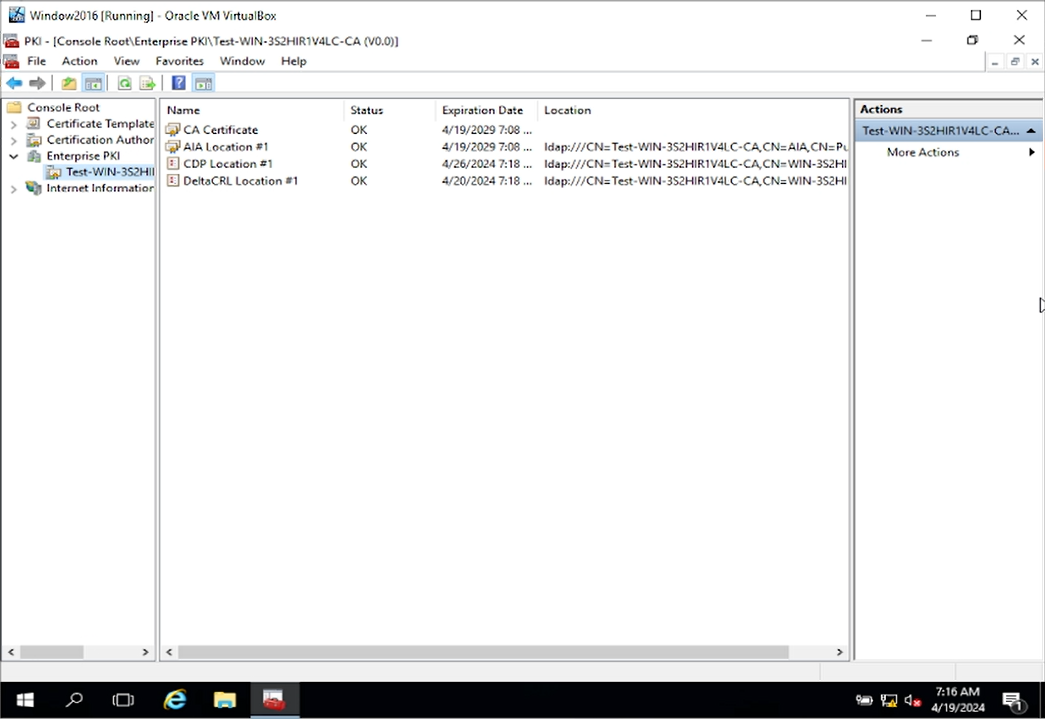
\includegraphics[width=0.8\linewidth]{figure//chapter4//lab4_1/ca_cert.png}
    \caption{Màn hình thông tin trong Enterprise PKI}
    \label{fig:enter-label}
\end{figure}

\begin{figure}[!htb]
    \centering
    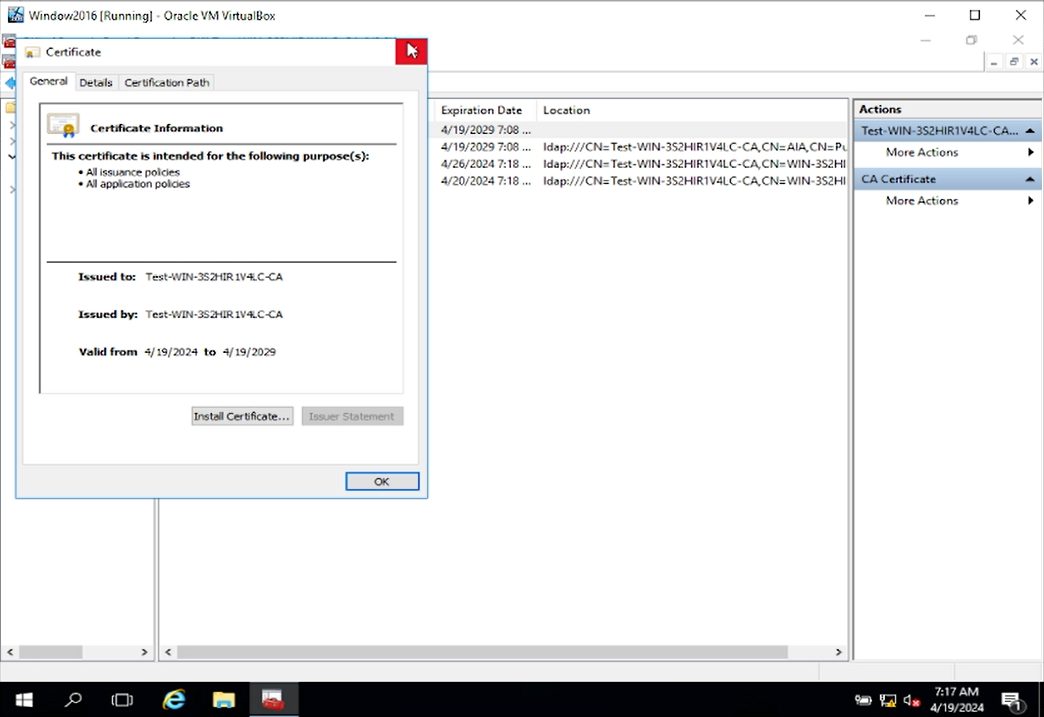
\includegraphics[width=0.8\linewidth]{figure//chapter4//lab4_2/ca_cert_info.png}
    \caption{Thông tin của CA Certificate}
    \label{fig:enter-label}
\end{figure}

\newpage
\noindent {\bf{Bước 3:}} Mở rộng phần \textbf{Certification Authority (Local)} và chọn ServerName. Sau đó chọn các certificate và các mục khác để biết thêm thông tin.

\begin{figure}[!htb]
    \centering
    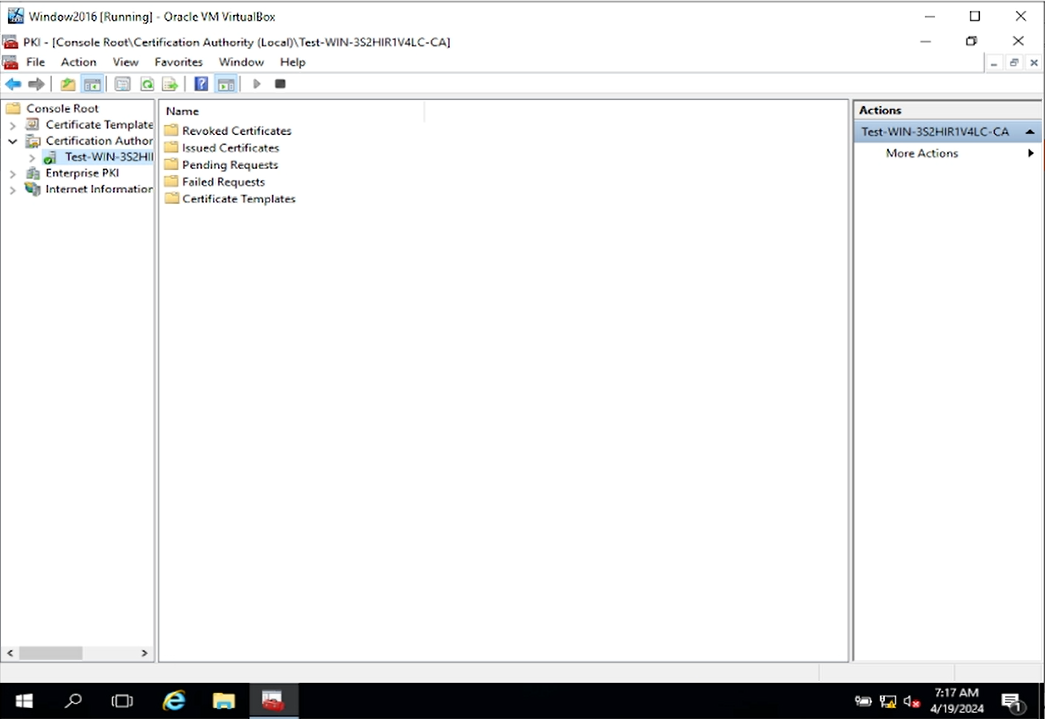
\includegraphics[width=0.9\linewidth]{figure//chapter4//lab4_2/ca_local.png}
    \caption{Thông tin trong Certification Authority (Local)}
    \label{fig:enter-label}
\end{figure}

\noindent {\bf{Bước 4:}} Mở rộng phần \textbf{Certificate Templates} ở trong mục Certification Authority (Local)/ServerName. Mở rộng các file này và tìm hiểu.

\begin{figure}[!htb]
    \centering
    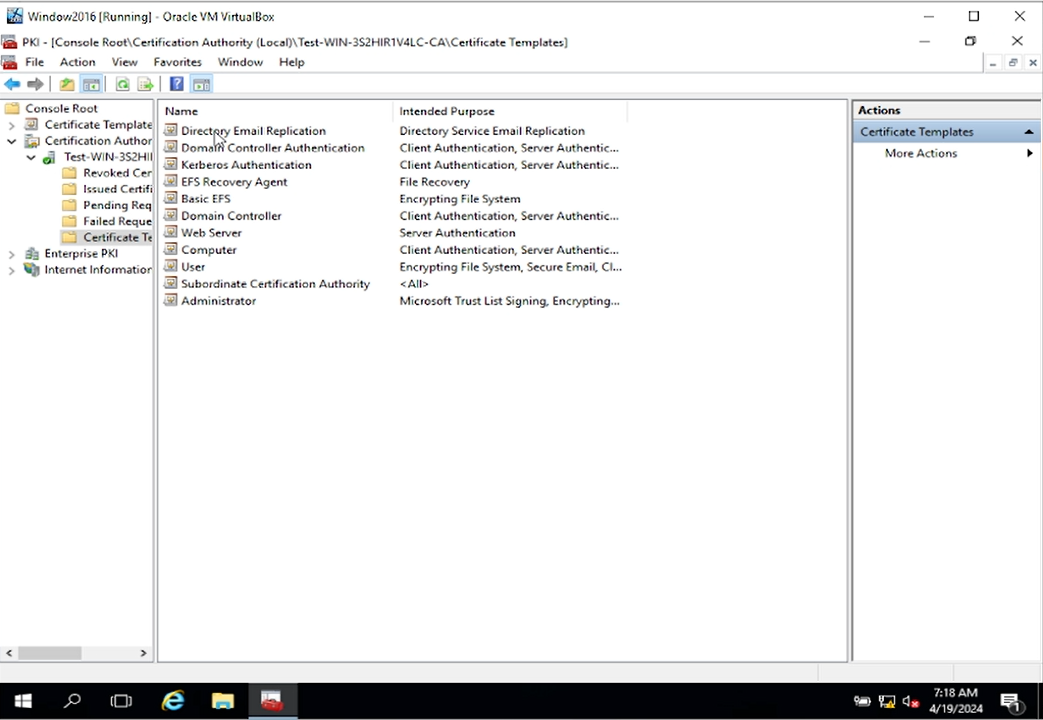
\includegraphics[width=0.9\linewidth]{figure//chapter4//lab4_2/cert_temp.png}
    \caption{Thông tin trong Certificate Templates}
    \label{fig:enter-label}
\end{figure}

\noindent {\bf{Bước 5:}} Vào Start, chọn \textbf{Windows Administrative Tools}, chọn \textbf{Internet Information Services (IIS) Manager}. Ở thanh Connection, chọn ServerName, mở rộng Sites và Default Web Site.

\begin{figure}[!htb]
    \centering
    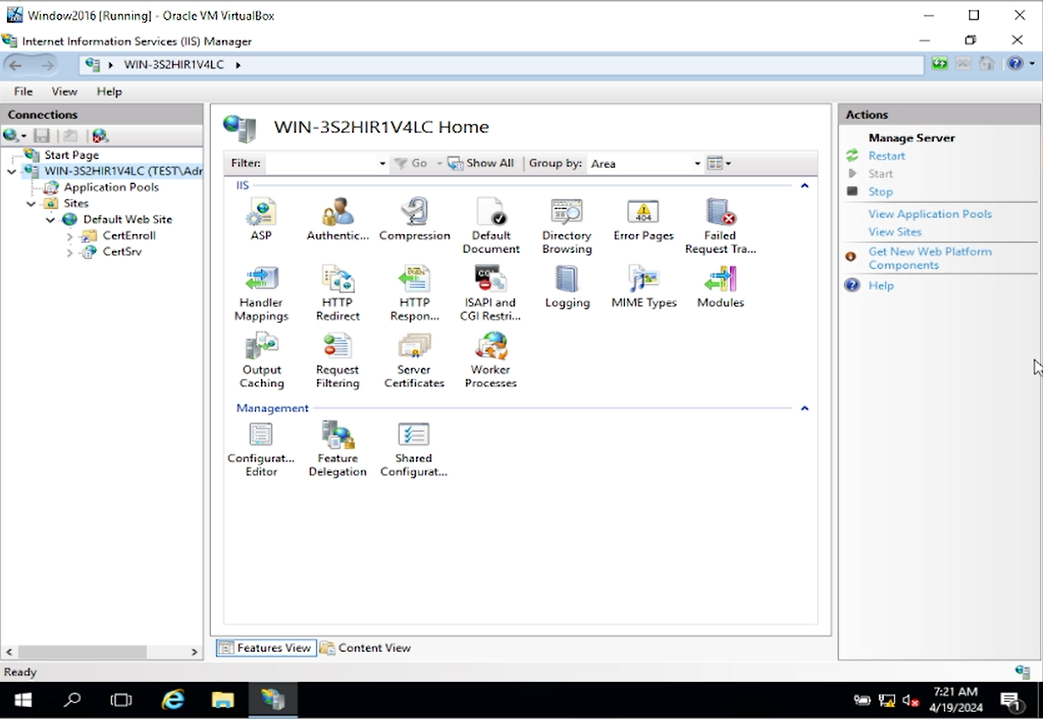
\includegraphics[width=0.9\linewidth]{figure//chapter4//lab4_2/iis_manager.png}
    \caption{Thông tin trong IIS Manager}
    \label{fig:enter-label}
\end{figure}

\noindent {\bf{Bước 6:}} Chọn Authentication. Chắc chắn rằng \textbf{Anonymous Authentication} đã được bật.

\begin{figure}[!htb]
    \centering
    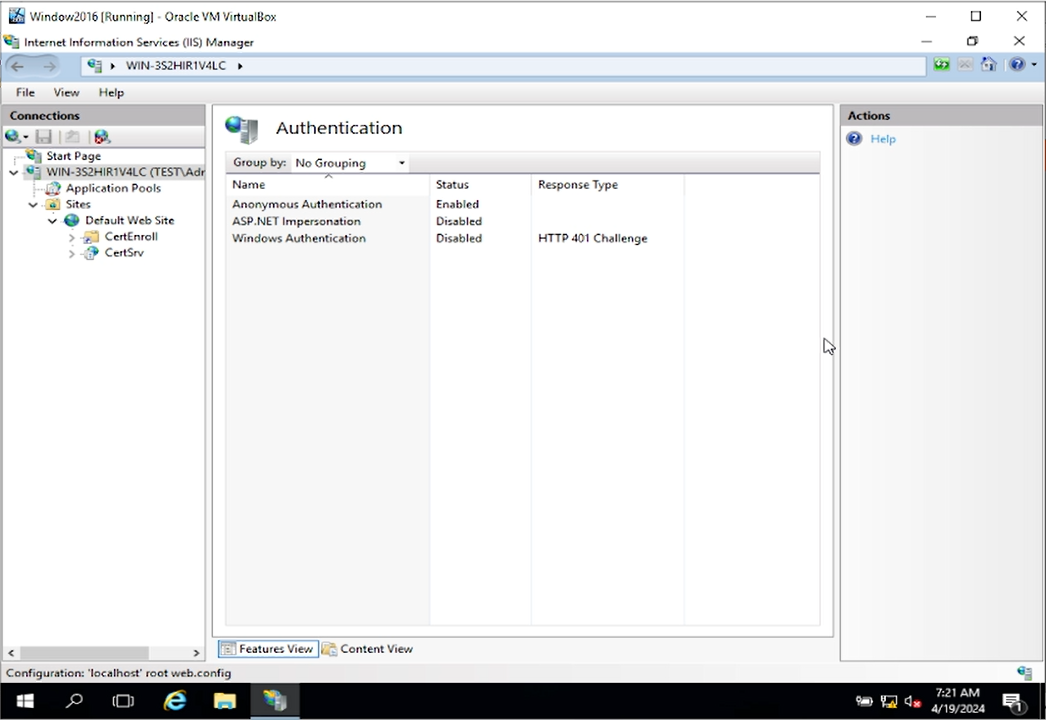
\includegraphics[width=0.8\linewidth]{figure//chapter4//lab4_2/iis_auth.png}
    \caption{Màn hình Authentication trong IIS Manager}
    \label{fig:enter-label}
\end{figure}

\newpage
\noindent {\bf{Bước 7:}} Chọn \textbf{Default Web Site}, chọn \textbf{Authentication}. Kiểm tra \textbf{Anonymous Authentication}. Sau đó quay lại, chọn \textbf{SSL Settings}.

\begin{figure}[!htb]
    \centering
    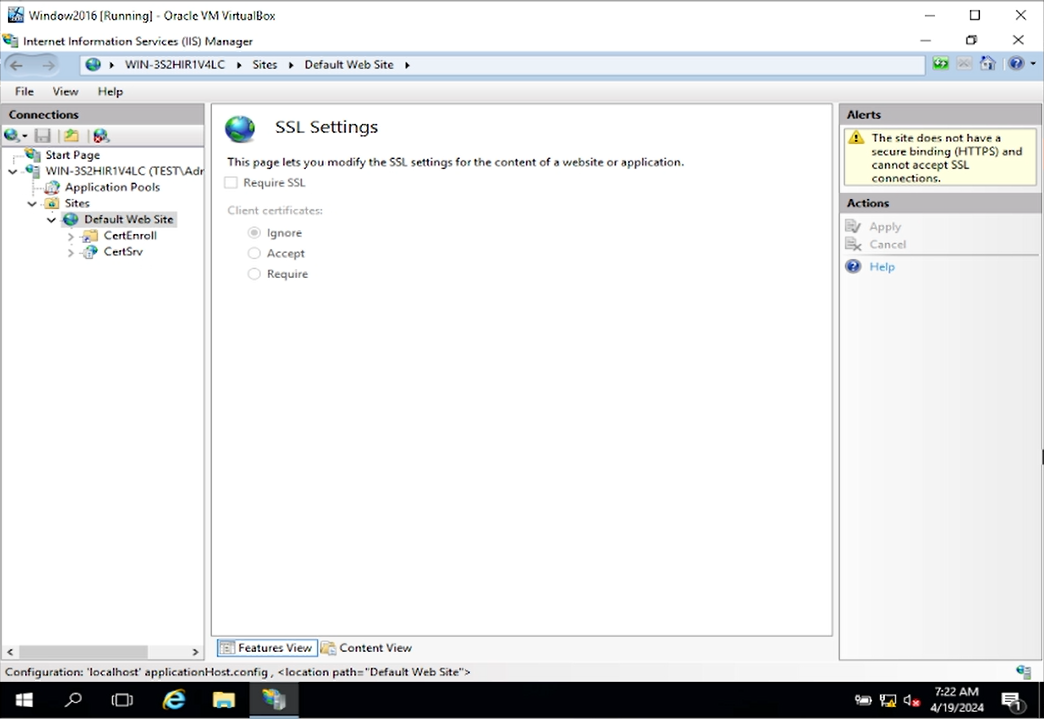
\includegraphics[width=0.8\linewidth]{figure//chapter4//lab4_2/ssl_settings.png}
    \caption{Màn hình SSL Settings}
    \label{fig:enter-label}
\end{figure}

\noindent Tại đây, bạn có thể thấy các mục bị mờ đi. Lý do là bởi đang không có binding HTTPS và web server certificate tới port 443. Để thêm binding, ta chọn vào ServerName, chọn Server Certificates. Trong trường hợp chỉ có 1 certificate, reboot máy ảo. Sau đó, ta có thể nhấn vào các certificate để biết thêm thông tin.

\begin{figure}[!htb]
    \centering
    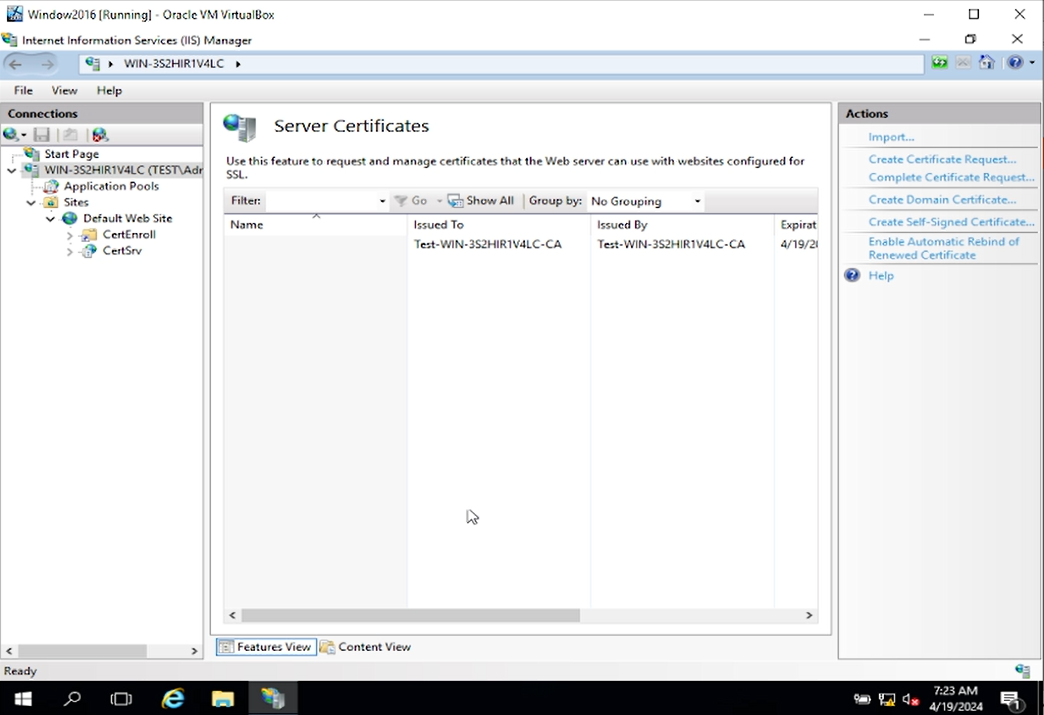
\includegraphics[width=0.8\linewidth]{figure//chapter4//lab4_2/ser_cert.png}
    \caption{Các certificate trong Server Certificates}
    \label{fig:enter-label}
\end{figure}

\newpage

\noindent {\bf{Bước 8:}} Chọn \textbf{Default Web Site}. Chọn \textbf{Bindings} ở thanh \textbf{Actions} ở phía bên phải.

\begin{figure}[!htb]
    \centering
    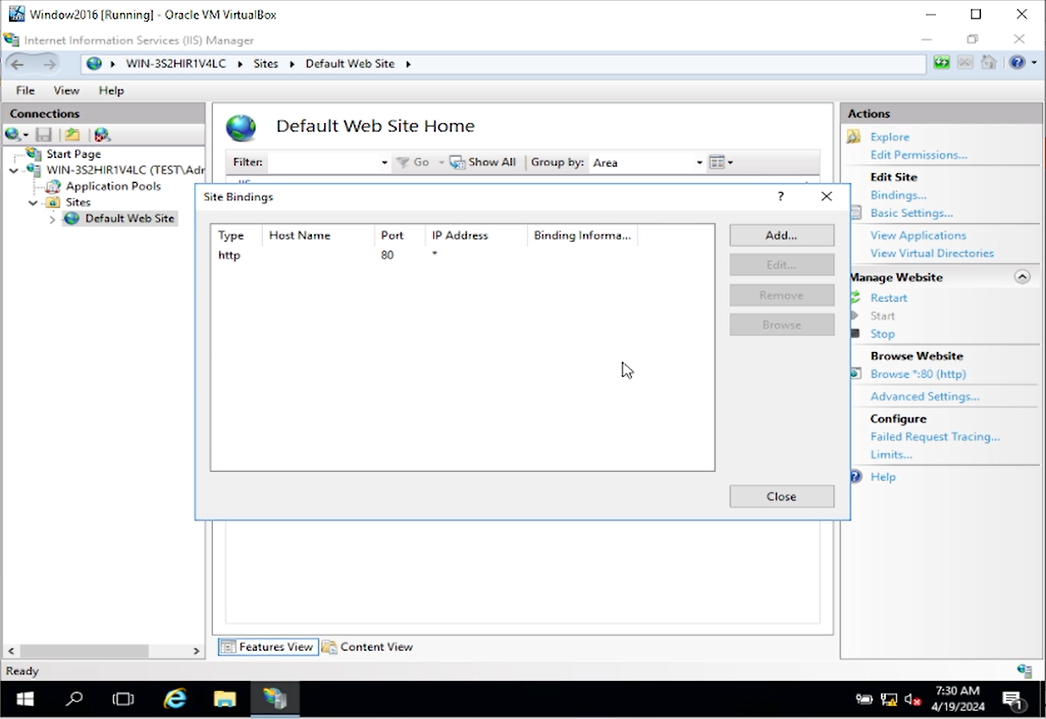
\includegraphics[width=0.9\linewidth]{figure//chapter4//lab4_2/bindings.png}
    \caption{Màn hình Bindings}
    \label{fig:enter-label}
\end{figure}

\noindent {\bf{Bước 9:}} Chọn \textbf{Add}, chọn \textbf{https} ở \textbf{Type} cho port 443. Chọn SSL Certificates tương ứng với ServerName. Click \textbf{OK}.

\begin{figure}[!htb]
    \centering
    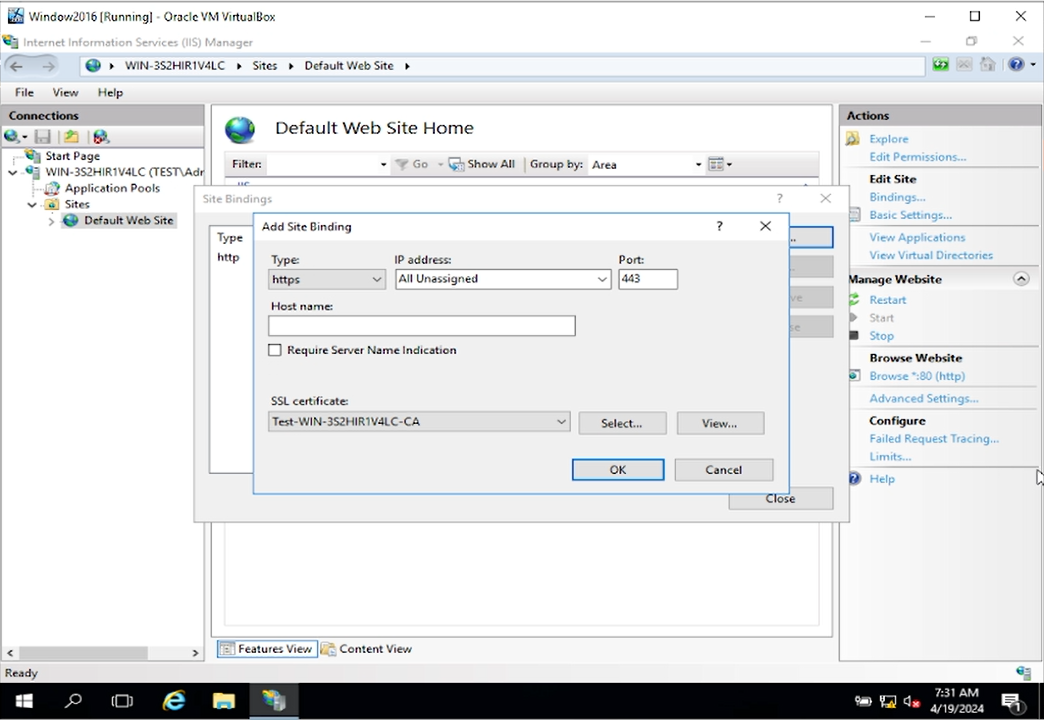
\includegraphics[width=0.9  \linewidth]{figure//chapter4//lab4_2/add_bindings.png}
    \caption{Thêm Binding}
    \label{fig:enter-label}
\end{figure}

\noindent {\bf{Bước 10:}} Quay lại \textbf{SSL Settings} trong \textbf{Default Web Site}. Lúc này các mục không còn mờ nữa. Chọn \textbf{Require SSL} và nhấn \textbf{Apply}.

\begin{figure}[!htb]
    \centering
    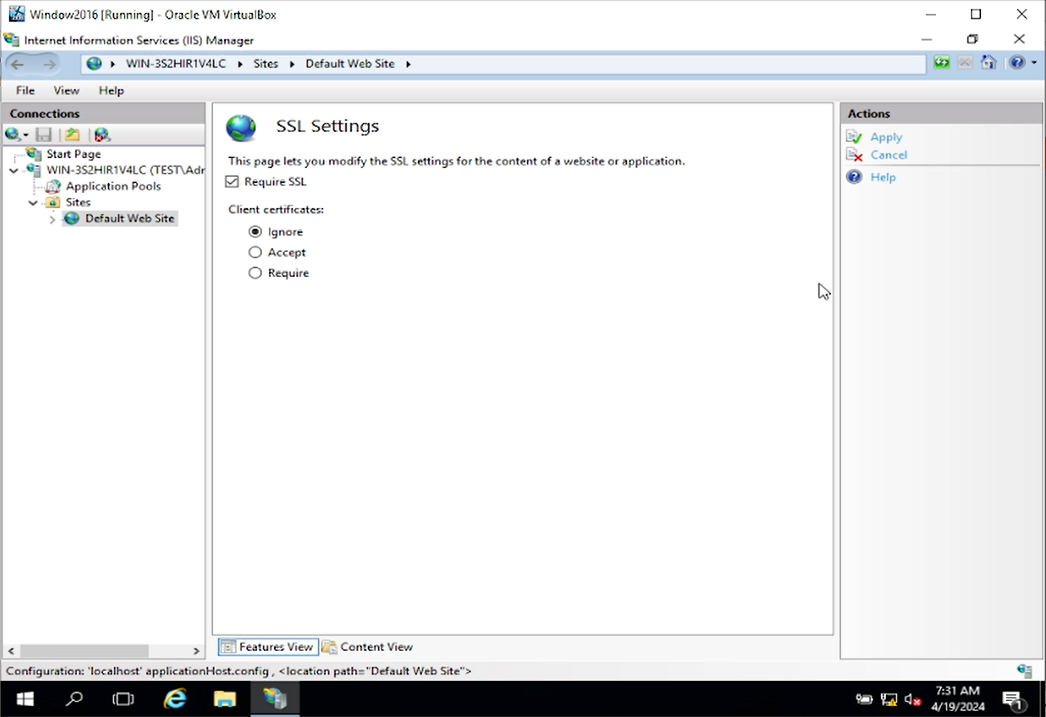
\includegraphics[width=0.9\linewidth]{figure//chapter4//lab4_2/ssl_setting_after_bind.png}
    \caption{Màn hình SSL Settings sau khi thực hiện thêm Binding}
    \label{fig:enter-label}
\end{figure}

\noindent {\bf{Bước 11:}} Vào \textbf{Start}, chọn \textbf{Active Directory Users and Computers}. Sau đó tạo người dùng mới. Đặt tên là Anthony Newman, username là anewman, mật khẩu là Pa\$\$word. Sau đó click vào tài khoản của Anthony Newman và điền email là anewman@teamx.net. 

\begin{figure}[!htb]
    \centering
    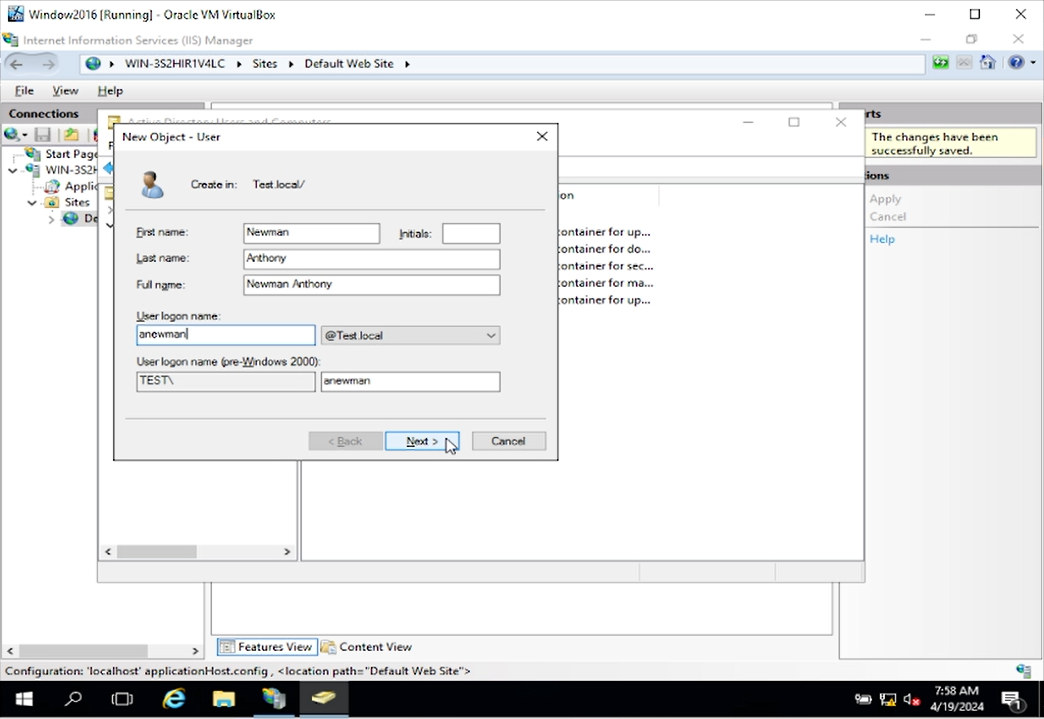
\includegraphics[width=0.8\linewidth]{figure//chapter4//lab4_2/create_account.png}
    \caption{Tạo người dùng mới}
    \label{fig:enter-label}
\end{figure}

\subsection{Review Questions}

\noindent Câu 1: 

D: The client and web server exchanging root certificates.

\noindent Câu 2: 

D: 443.

\noindent Câu 3: 

D: No port had been configured to "listen" for https requests.

\noindent Câu 4: 

C: To have a location for centralized account maintenance.

\noindent Câu 5: True.